\documentclass[a4paper, 11pt]{article}

% Locale/encoding with XeTeX: UTF-8 by default, use fontspec
\usepackage{unicode-math}
\usepackage{polyglossia} % Modern replacement for Babel
\setmainlanguage{english}
\usepackage{csquotes} % guillemets
\usepackage{listings}
% Other
\usepackage{fullpage}
\usepackage{graphicx}
%\usepackage{enumerate}
%\usepackage{graphicx}
\lstset{language=Lisp}   
\begin{document}

\title{Final report on the Digital Systems course project}
\author{Nguyễn Lê Thành Dũng \and Thomas Bourgeat}

\maketitle

\section{Summary}

The project's objectives were to design a synchronous circuit usable as a general-purpose processor, and to simulate this processor at the logic gate level using a simulator we wrote ourselves. In the end, blah clock qmlkdsfj.
Those objectives have been met.

Since there's a lot to say here, we will refer you to our two previous intermediate reports for information on the work we did previously.

What follows here is a high-level view of our architecture, combined with a rough description of how we developed the processor. All the details are confined to the appendices.

\section{What's new since last time}

\begin{itemize}
\item In the simulator, we fixed some bugs, and added all the features needed in order to run our processor at a reasonable performance and make the clock demo work. More details in Appendix foobar.
\item In our report on the processor design, we described the kind of architecture we wanted to implement and the rough shape of its machine language. Since then, we have kept the same ideas and filled in the details, following the plans we sketched in that report to their completion.
\item 
\end{itemize}



\section{Designing an instruction set}

First, we needed to fix an instruction set that would be expressive enough for our purposes, that is, writing a clock. We concurrently developed, in a single OCaml file, a syntax tree for the S-code (our assembly language), an interpreter for this language, and a program which would count seconds and minutes. 

Our interpreter was meant as a model of what 

\section{From an imperative S-code interpreter to hardware}




\newpage
\appendix

\section{Mini-Lisp and S-Code illustrated through the clock program}


\begin{lstlisting}
(defun main ()
  (count-hours 18))

(defun count-seconds (sec)
  (print-second sec)
  (let ((new-sec (+1 sec)))
    (if (>=60? new-sec)
        ()  
        (synchronize (count-seconds new-sec)))))

(defun count-minutes (min)
  (print-minute min)
  (count-seconds 0)
  (let ((new-min (+1 min)))
    (if (>=60? new-min)
        ()  
        (synchronize (count-minutes new-min)))))
\end{lstlisting}

\newpage
\section{Functional units in the processor}
\subsection{ALU}
\begin{figure}[h]
\center
\caption{Schematic of the ALU}
   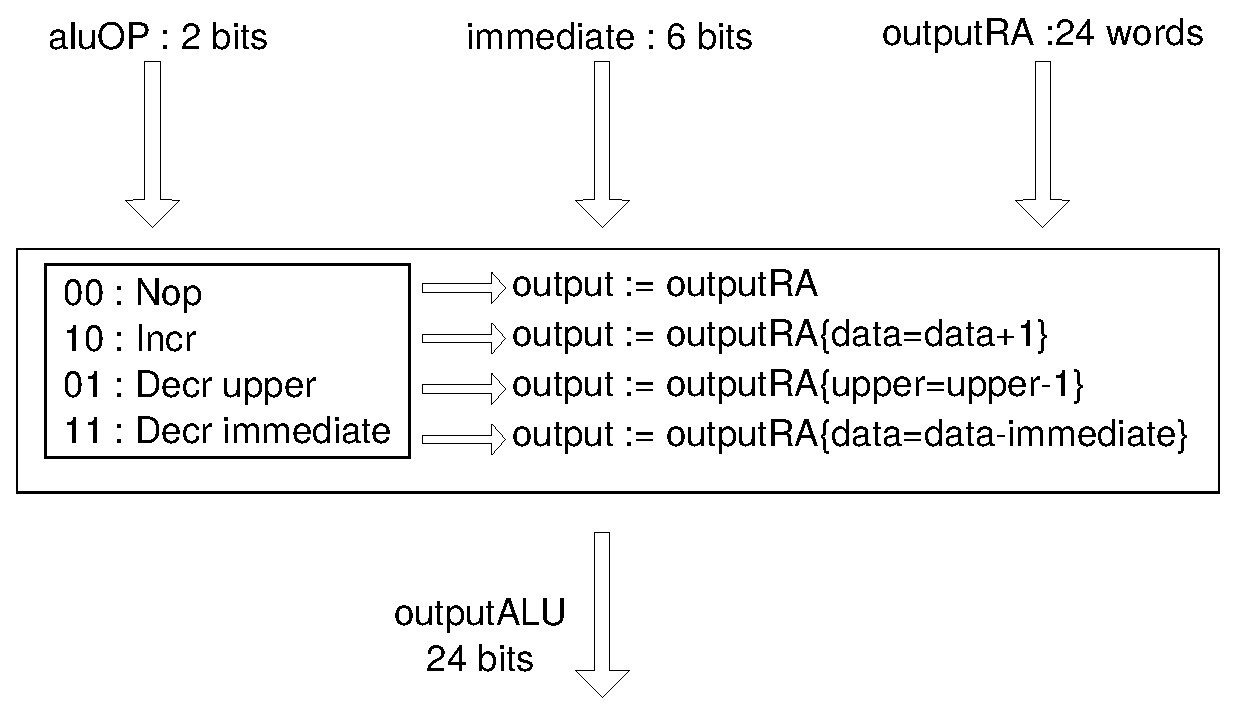
\includegraphics[scale=0.5]{ALU.eps}
\end{figure}

\newpage
\subsection{Memory system}
\begin{figure}[h]
\center
\caption{Schematic of the memory system}
   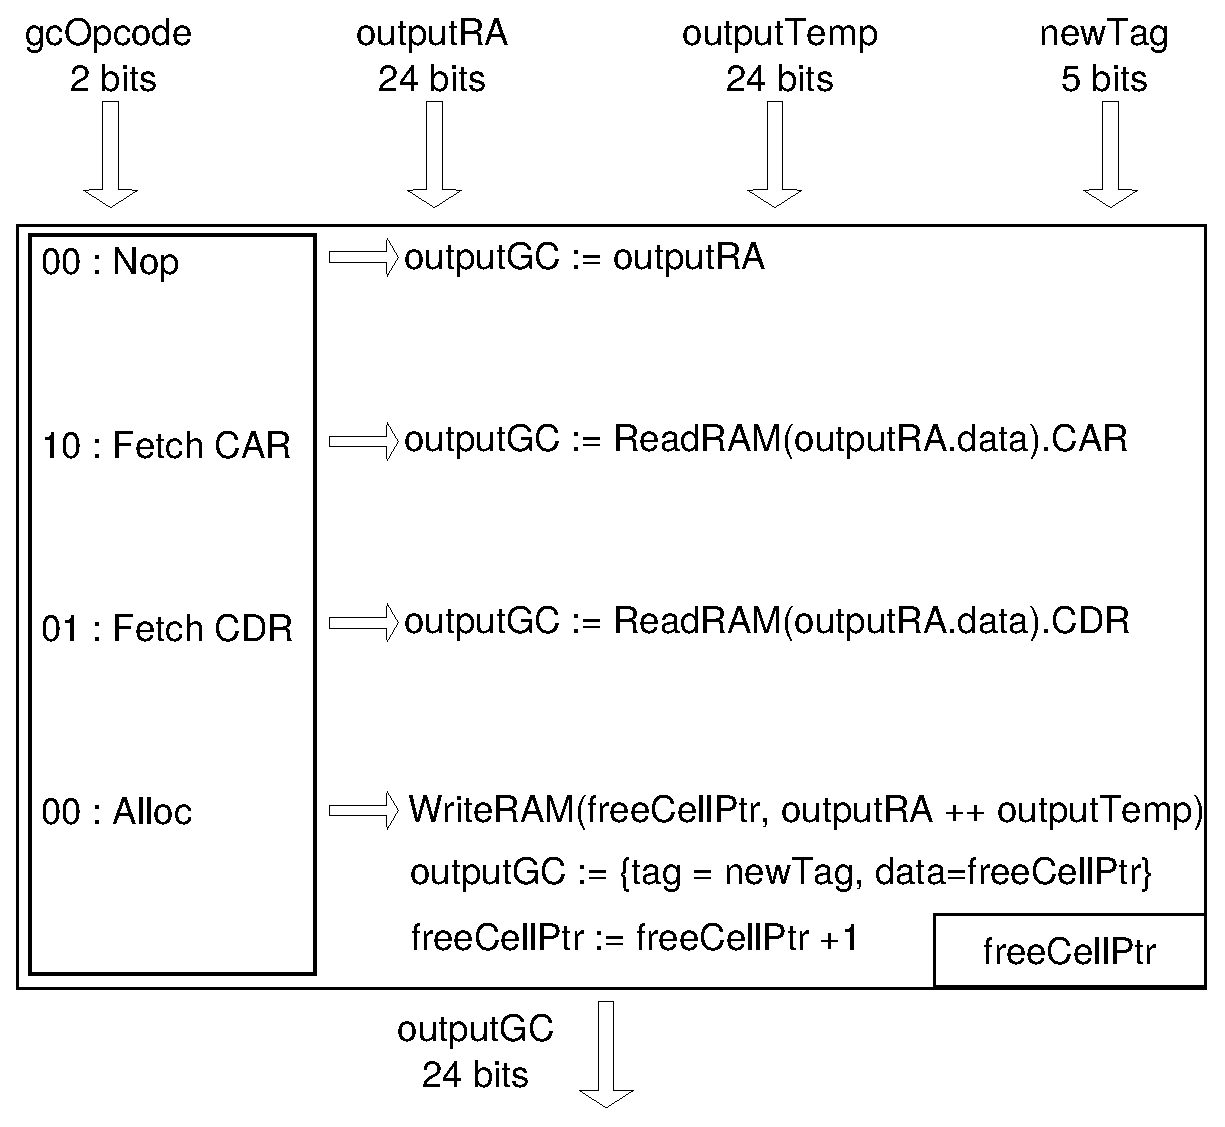
\includegraphics[scale=0.5]{GC.eps}
\end{figure}
\newpage
\subsection{Register Array}
\begin{figure}[h]
\center
\caption{Schematic of the register array}
   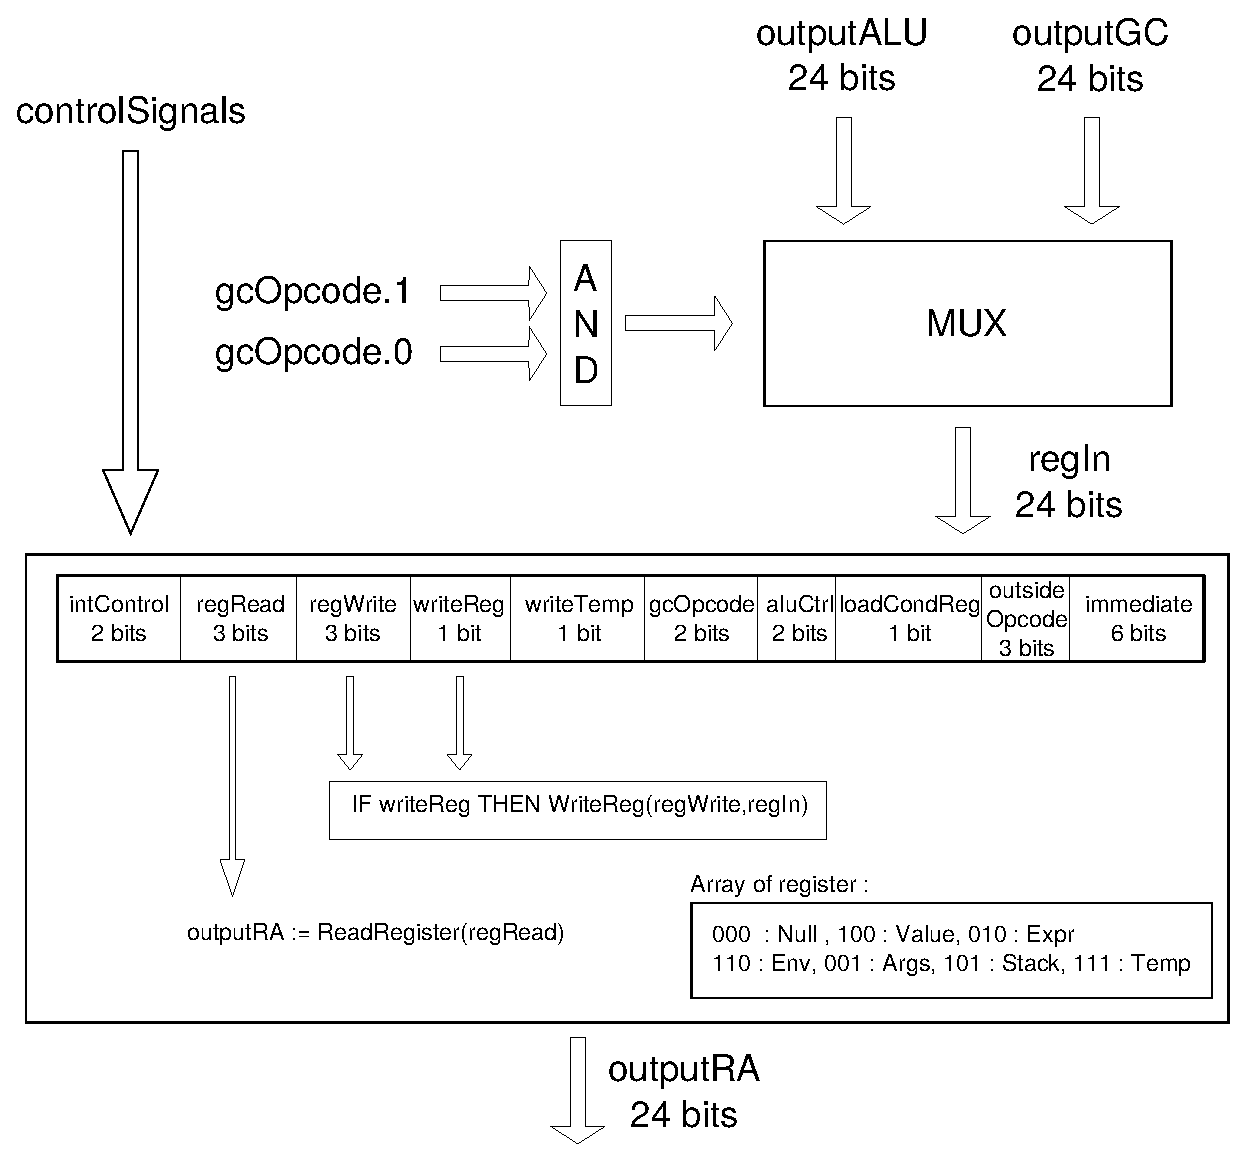
\includegraphics[scale=0.5]{RA.eps}
\end{figure}
\newpage
\subsection{Control unit}
\begin{figure}[h]
\center
\caption{Schematic of the control unit}
   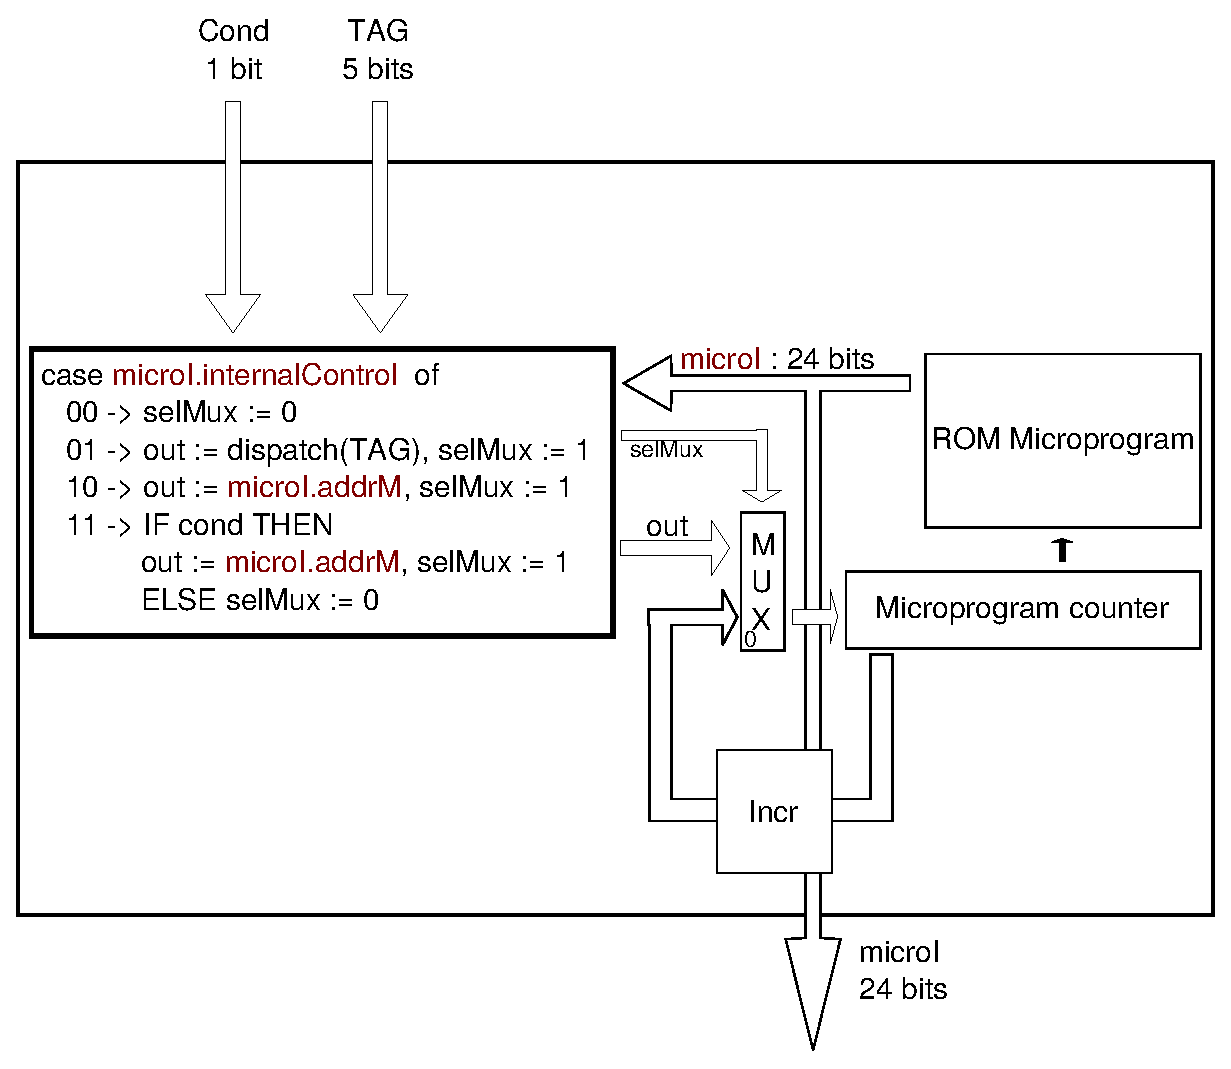
\includegraphics[scale=0.5]{control.eps}
\end{figure}


\section{The microprogram}


\section{The Caillou netlist description language}


\section{Source files in the project}
\begin{itemize}
\item "README.md" : Self describing
\item "build.sh" : a script to build the entire project. It generates : rom,
simulator and processor.net. See the README for more precisions.
\end{itemize}
\subsection{./haskell}

\subsection{./ocaml}

\subsection{./report}
\begin{itemize}
\item Your struly
\end{itemize}


\bibliographystyle{plain}
\bibliography{biblio}

\end{document}
